\documentclass[10pt]{article}
\usepackage[letterpaper, margin=1in]{geometry}
\usepackage[pdftex]{graphicx}
\usepackage[utf8]{inputenc}
\usepackage{tikz, wrapfig, amssymb, array, mathtools, circuitikz, physics, parskip, hyperref}
\usepackage{enumerate}
\usepackage{tkz-euclide}
\usepackage{titlesec}
\usepackage{lipsum}
\usepackage[english]{babel}
\usepackage{amsmath, amsthm}
\usepackage{fancyhdr}
\usepackage{xcoffins}
% \usepackage{dirtytalk}
\usepackage{tcolorbox}
\usepackage{../local}



\title{\code Homework}
\author{Yutong Du}

\newcommand{\code}{Physics 137A}
\newcommand{\class}{Quantum Mechanics}
\linespread{1.1}

\renewcommand{\maketitle}{%
\hrule height4pt
\large{Eric Du \hfill \code}\\
\large{HW 03} \Large{\hfill \class \hfill} \large{\today}
\hrule height4pt \vskip .7em
}

\begin{document}
\maketitle

    \section*{Collaborators}

    I worked with \textbf{Andrew Binder} to complete this homework. I also thank him for his Ti\textit kZ diagrams.
    \section*{Problem 1}


    Calculate $\frac{\dd \mean{p}}{\dd t}$

    \begin{solution}

  
        We compute the derivative of the expectation value:

        \begin{align*}
          \frac{\dd\mean{p}}{\dd t} &= \frac{\dd}{\dd t}\left[-i\hbar\infint\left(\Psi^\star\frac{\partial\Psi}{\partial x}\right)\dx\right] = -i\hbar\infint\frac{\partial}{\partial t}\left(\Psi^\star\frac{\partial \Psi}{\partial x}\right)\dx\\
          &= -i\hbar\infint \frac{\partial\Psi}{\partial x}\frac{\partial\Psi^\star}{\partial t} + \Psi^\star\frac{\partial}{\partial x}\frac{\partial \Psi}{\partial t}\dx\\
          &= -i\hbar\infint \frac{\partial\Psi}{\partial x}\left(-\frac{i\hbar}{2m}\frac{\partial^2\Psi^\star}{\partial x^2} + \frac{i}{\hbar}V\Psi^\star\right)+ \Psi^\star\frac{\partial}{\partial x}\left(\frac{i\hbar}{2m}\frac{\partial^2\Psi}{\partial x^2} - \frac{i}{\hbar}V\Psi\right)\dx\\
          &= -i\hbar\infint\frac{i\hbar}{2m}\left(\Psi^\star \frac{\partial^3\Psi}{\partial x^3} - \frac{\partial^2\Psi^\star}{\partial x^2}\frac{\partial\Psi}{\partial x}\right) + \frac{i}{\hbar}\left(V\Psi^\star\frac{\partial\Psi}{\partial x} - \Psi^\star\frac{\partial}{\partial x}(V\Psi)\right)\dx
        \end{align*}

        To compute the first term, we take two partial derivatives and we find that it's equal to zero (there is simply way too much algebra for me to write it all out, this was also confirmed via computer). Now let's simplify the second term:


        \[V\Psi^\star\frac{\partial \Psi}{\partial x} - \Psi^\star\frac{\partial}{\partial x}(V\Psi) = V\Psi^\star\frac{\partial\Psi}{\partial x} - \Psi^\star \left( V\frac{\partial\Psi}{\partial x} - \frac{\partial V}{\partial x}\Psi \right)= -|\Psi|^2\frac{\partial V}{\partial x}\]

        So putting this back into our integral: 
        \[\frac{\dd\mean{p}}{\dd t} = -i\hbar\int\frac{i}{\hbar}\left(-|\Psi|^2\frac{\partial V}{\partial x}\right) = \int\Psi^\star\left(-\frac{\partial V}{\partial x}\right)\Psi = \fbox{$\mean{-\frac{\partial V}{\partial x}}$}\]
        
        And thus we have shown that 

        \[ \frac{\dd \mean p}{\dd t} = \mean{- \frac{\partial V}{\partial x}}\]
        
        As desired. $\blacksquare$
    \end{solution}
    \pagebreak
    \section*{Problem 2}

    Suppose you wanted to describe an \textbf{unstable particle}, that spontaneously disintegrates with ``lifetime'' r. In that case the total probability of finding the particel somewher should \textit{not} be constant, but should decrease at (say) an exponential rate. 

    \[ P(t) \equiv \infint \left| \Psi(x, t)\right|^2 \dx = e^{-1/\tau}\]

    A crude way of achieving this result is as follows. In equation 1.24 we tacitly assumed that $V$ (the potential energy) is \textit{real}. That is certainly reasonable, but it leads to the ``conservation of probability" enshrined in Equation 1.27. What if we assign to $V$ an imaginary part: 

    \[ V = V_0 - i\Gamma\] 

    where $V_0$ is the true potential energy and $\Gamma$ is a positive real constant?

    \begin{enumerate}[(a)]
        \item Show that (in place of Equation 1.27) we now get
        \[ \frac{\dd P}{\dd t} = -\frac{2\Gamma}{h} P\]
        \begin{solution}
            Following the instructions, we let $V = V_0 - i\Gamma$. Now we calculate $P(t)$:
            
            \[\frac{\dd P}{dt} = \infint \frac{\partial}{\partial t} |\Psi(x, t)|^2 \dx\]

            We take the product rule:

            \[ \frac{\dd P}{dt} = \infint \left(\frac{\partial \Psi}{\partial t} \Psi^\star + \frac{\partial \Psi^\star}{\partial t} \Psi\right) \dx\]

            We need the values $\frac{\partial \Psi}{\partial t}$ and $\frac{\partial \Psi^\star}{\partial t}$. We will get these from the \schrodinger equation. Now we let $V = V_0 - i\Gamma$. This means that our equations for $\frac{\partial \psi}{\partial t}$ and $\frac{\partial \psi^\star}{\partial t}$ become:

            \begin{align*}
                \frac{\partial \Psi}{\partial t} &= \frac{i\hbar}{2m} \frac{\partial^2\Psi}{\partial x^2} - \frac{i}{\hbar}(V_0 - i\Gamma)\Psi\\
                \frac{\partial \Psi^\star}{\partial t} &= -\frac{i\hbar}{2m} \frac{\partial^2 \Psi^\star}{\partial x^2} + \frac{i}{\hbar}(V_0 + i\Gamma)\Psi
            \end{align*}

            So therefore

            \begin{align*}
                \frac{\partial}{\partial t} |\Psi|^2 &= \Psi^\star\left[\frac{i\hbar}{2m} \frac{\partial^2\Psi}{\partial x^2} - \frac{i\Psi}{\hbar}(V_0 - i\Gamma)\right] + \Psi\left[\frac{-i\hbar}{2m} \frac{\partial^2\Psi^\star}{\partial x^2} + \frac{i\Psi^\star}{\hbar}(V_0 + i\Gamma)\right]\\
                &= \frac{i\hbar}{2m}\left(\frac{\partial^2 \Psi}{\partial x^2} \Psi^\star - \frac{\partial^2\Psi^\star}{\partial x^2}\Psi\right) - \frac{i\Psi\Psi^\star}{\hbar}(V_0 - i\Gamma - (V_0 + i\Gamma))\\
                &= \frac{i\hbar}{2m}\left(\frac{\partial^2 \Psi}{\partial x^2}\Psi^\star - \frac{\partial^2\Psi^\star}{\partial x^2}\Psi\right) - 2\Gamma \frac{\Psi\Psi^\star}{\hbar}
            \end{align*}

            Taking the integral of this, it's shown in the textbook that the first term drops to zero when evaluated. Now notice the second term:

            \[ \infint -2\Gamma \frac{\Psi \Psi^\star}{\hbar} = \frac{-2\Gamma}{\hbar} \infint |\Psi|^2 \dx = \frac{-2\Gamma}{\hbar} P\]
        \end{solution}
        \item Solve for $P(t)$, and find the lifetime of the particle in terms of $\Gamma$.
        
        \begin{solution}
            We have the equation from part (a). We can perform a separation of variables:

            \begin{align*}
                \frac{1}{P} \dd P &= -\frac{2\Gamma}{\hbar} \dd t\\
                \ln P &= -\frac{2\Gamma}{\hbar} + C\\
                \therefore P(t) &= Ae^{-2\Gamma t/\hbar}
            \end{align*}

            We don't have enough information to solve for $A$, but it doesn't matter here since the question doesn't ask for it. Since $P(t)$ is in the form of  $e^{-1/\tau}$, this means that

            \[ \tau = \frac{\hbar}{2\Gamma}\]
            
            For our derived expression of $P(t)$.

        \end{solution}
    \end{enumerate}


    \pagebreak

    \section*{Problem 3}

    Calculate the following commutators:

    \begin{enumerate}[(a)]
        \item $[\hat x, \hat x]$

        \begin{solution}
            The commutator of any operator with itself is equal to zero, and this is no exception.
        \end{solution}
        \item $[\hat x, \hat p]$

        \begin{solution}
            From lecture, we know that $[\hat x, \hat p] = i\hbar$. 
        \end{solution}
        \item $[\hat x^2, \hat p]$

        \begin{solution}
            We act the commutator on an arbitrary function $f(x)$:

            \begin{align*}
                [\hat x^2, \hat p]f(x) &= \left[-x^2i\hbar \frac{\partial}{\partial x} + i\hbar \frac{\partial}{\partial x}x^2\right] f(x)\\
                &= -x^2\hbar \frac{\partial}{\partial x} f(x)+ i\hbar \frac{\partial}{\partial x}(x^2f(x))\\
                &= -x^2i\hbar \frac{\partial f}{\partial x} + i\hbar\left[x \frac{\partial f}{\partial x} + x^2 \frac{\partial f}{\partial x}\right]\\
                &= i\hbar x \frac{\partial f}{\partial x} = -\hat x\hat p
                \therefore [\hat x^2, \hat p] = -\hat x\hat p
            \end{align*}
        \end{solution}
        \item $[\hat x, f(\hat x)]$
        
        \begin{solution}
            \begin{align*}
                [\hat x, f(\hat x)]g(x) &= (xf(\hat x) - f(\hat x)x)g(x)\\
                &= xf(x)g(x) - f(x)xg(x) = 0
            \end{align*}

            The last step is true since $f(\hat x) = f(x)$.
        \end{solution}
        \item $[\hat p, f(\hat x)]$
        \begin{solution}
            \begin{align*}
                    [\hat p, f(\hat x)]g(x) &= \left(\hat p f(\hat x) - f(\hat x)\hat p\right)g(x)\\
                    &= \hat p f(x)g(x) - f(x) \hat pg(x)\\
                    &= -i\hbar\left(\frac{\partial f}{\partial x}g(x) + \frac{\partial g}{\partial x} g(x)\right)\\
                    &= -i\hbar\left(\frac{\partial f}{\partial x} g(x) + \frac{\partial g}{\partial x}f(x) \right) + f(x) i\hbar \frac{\partial g}{\partial x}\\
                    &= -i\hbar \frac{\partial f}{\partial x} - i\hbar \frac{\partial g}{\partial x} + i\hbar f(x) \frac{\partial g}{\partial x}\\
                    &= -i\hbar\frac{\partial f}{\partial x} g(x)\\
                    \therefore [\hat p, f(\hat x)] = -i\hbar \frac{\partial f}{\partial x} &= \hat p f(\hat x)
            \end{align*}

           
        \end{solution}
        \item $[\hat x, \hat H]$ for general potential $V(x)$
        
        \begin{solution}

            We know that $\hat H = \frac{\hat p^2}{2m} + V(x)$, so we can compute this using brute force algebra: 
            \begin{align*}
                [\hat x, \hat H]f(x) &= \hat x \left(\frac{\hat p^2}{2m} f(x) + V(x)f(x)\right) - \left(\frac{\hat p^2}{2m}xf(x) + V(x)xf(x)\right)
            \end{align*}

            Since $\frac{\hat p^2}{2m} f(x) = -\frac{i\hbar}{2m} \frac{\partial f}{\partial x}$ so this simplification gives:

            \begin{align*}
              [\hat x, \hat H]f(x)&= \hat x \left(-\frac{i\hbar}{2m} \frac{\partial f}{\partial x} + V(x)f(x)\right) - \frac{i\hbar}{2m} \frac{\partial}{\partial x}(xf(x)) - V(x) xf(x)\\
                &= -x\frac{i\hbar}{2m} \frac{\partial f}{\partial x} - \frac{i\hbar}{2m}\left(f(x) + \frac{\partial f}{\partial x}\right)\\
                &= -\frac{i\hbar}{2m} f(x)
            \end{align*}

            Therefore $[\hat x, \hat H] = -\frac{i\hbar}{2m}$.
        \end{solution}
    \end{enumerate}

    \pagebreak
    \section*{Problem 4}

    Consider the following potential $V(x)$:

    \[\begin{tikzpicture}[scale=2]
        \draw[thick, gray!70, -stealth] (-2.5,0) -- (2.5,0) node[anchor=west, color=black] {$x$};
        \draw[thick, gray!70, -stealth] (0,-0.75) -- (0,2.25) node[anchor=south, color=black] {$V(x)$};
        \draw[thick] (-2.5,2) -- (-1.5,2) -- (-1.5,-0.25) node[anchor=north] {$-b$} -- (-0.5,-0.25) node[anchor=north] {$-a$} -- (-0.5,1) -- (0.5,1) -- (0.5,-0.25) node[anchor=north] {$a$} -- (1.5,-0.25) node[anchor=north] {$b$} -- (1.5,2) -- (2.5,2);
        \node at (-0.1,-0.1) (o) {$0$};
        \node at (-0.25,-0.25) (v) {$V_0$};
        \node at (-0.25,1.25) (vv) {$V_1$};
        \node at (-0.25,2) (vvv) {$V_2$};
      \end{tikzpicture}\]


    We will be looking for solutions to the time-independent \schrodinger equation. 

    \begin{enumerate}[(a)]
        \item For what range of values $E$ 
        \begin{enumerate}[i.]
            \item are we certain there does not exist a solution?
            
            \begin{solution}
                Any $E < V_0$ has no solution.
            \end{solution}
            \item do we have solutions which are bound states?

            \begin{solution}
                Bound state solutions exist for $V_0 < E < V_2$.
            \end{solution}
            \item do we have solutions which are unbound states?
            
            \begin{solution}
                Unbound state solutions exist where $E > V_2$.
            \end{solution}
        \end{enumerate}
        \item Consider the case $V_0 < E < V_1$. Where are the classically allowed and disallowed regions? In other words, if a classical particle has total energy $E$, where is it possible or impossible for it to be?
        
        \begin{solution}
            The classically allowed solutions are those where $E > V(x)$. From here we can see that the allowed regions are:

            \[ x \in (-b, -a) \cup (a, b)\]

            Conversely, the disallowed regions would be the complement of this, so they are 
            
            \[x \in (-\infty, -b) \cup (-a, a) \cup (b, \infty)\]
        \end{solution}
        \item The two lowest energy solutions (i.e. the ground state and the first excited state) are sketched below:
        
        \[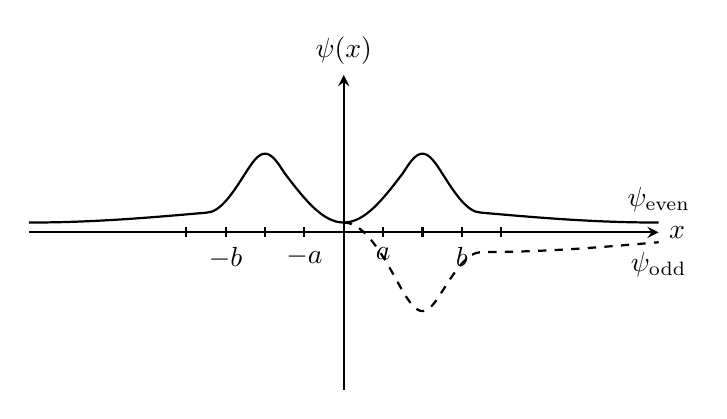
\begin{tikzpicture}
            \draw[thick, -stealth] (-4,0) -- (4,0) node[anchor=west] {$x$};
            \draw[thick, -stealth] (0,-2) -- (0,2) node[anchor=south] {$\psi(x)$};
            \draw[thick] (-0.5,0.0625) -- (-0.5,-0.0625) node[anchor=north] {$-a$};
            \draw[thick] (-1.5,0.0625) -- (-1.5,-0.0625) node[anchor=north] {$-b$};
            \draw[thick] (0.5,0.0625) -- (0.5,-0.0625) node[anchor=north] {$a$};
            \draw[thick] (1.5,0.0625) -- (1.5,-0.0625) node[anchor=north] {$b$};
            \draw[thick] (-1,0.0625) -- (-1,-0.0625);
            \draw[thick] (1,0.0625) -- (1,-0.0625);
            \draw[thick] (-2,0.0625) -- (-2,-0.0625);
            \draw[thick] (2,0.0625) -- (2,-0.0625);
            \draw[thick] (-4,0.125) cos (-1.75,0.25) cos (-1.25,0.75) sin (-1,1) cos (-0.75,0.75) sin (0,0.125) cos (0.75,0.75) sin (1,1) cos (1.25,0.75) sin (1.75,0.25) sin (4,0.125) node[anchor=south] {$\psi_{\text{even}}$};
            \draw[thick, dashed] (0,0.125) cos (0.75,-0.75) sin (1,-1) cos (1.25,-0.75) sin (1.75,-0.25) cos (4,-0.125) node[anchor=north] {$\psi_{\text{odd}}$};
          \end{tikzpicture}\]

        Which wavefunction, $\psi_{even}$ or $\psi_{odd}$ has a lower energy? Explain why qualitatively 

        \begin{solution}
            $\psi_{even}$ has a lower energy solution because it has no nodes, as opposed to $\psi_{odd}$, which has a node at $x = 0$. Furthermore, the even solution always corresponds to $n = 0$, which is the lowest energy state a quantum system can have.
        \end{solution}
        \item Sketch the third and fourth energy levels (i.e. the second and third excited states), assuing their energies still satisfy $V_0 < E < V_1$. Clearly label the two wavefunctions, as well as the locations of $\pm a$ and $\pm b$. 
        
        \begin{solution}
            Below, we have the sketches for the third and fourth energy levels:
            \[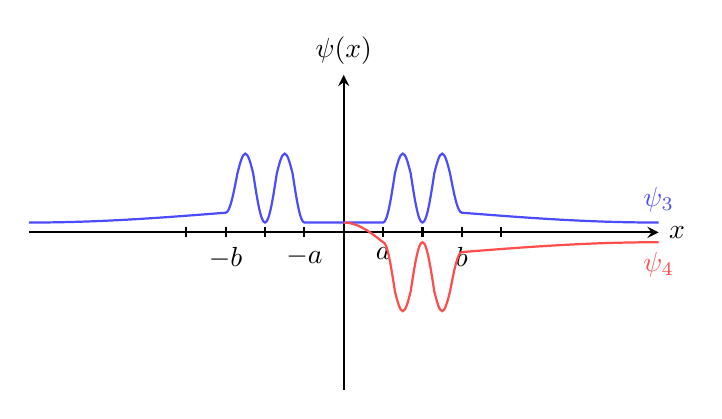
\begin{tikzpicture}
            \draw[thick, -stealth] (-4,0) -- (4,0) node[anchor=west] {$x$};
            \draw[thick, -stealth] (0,-2) -- (0,2) node[anchor=south] {$\psi(x)$};
            \draw[thick] (-0.5,0.0625) -- (-0.5,-0.0625) node[anchor=north] {$-a$};
            \draw[thick] (-1.5,0.0625) -- (-1.5,-0.0625) node[anchor=north] {$-b$};
            \draw[thick] (0.5,0.0625) -- (0.5,-0.0625) node[anchor=north] {$a$};
            \draw[thick] (1.5,0.0625) -- (1.5,-0.0625) node[anchor=north] {$b$};
            \draw[thick] (-1,0.0625) -- (-1,-0.0625);
            \draw[thick] (1,0.0625) -- (1,-0.0625);
            \draw[thick] (-2,0.0625) -- (-2,-0.0625);
            \draw[thick] (2,0.0625) -- (2,-0.0625);
            \draw[thick, blue!70] (-4,0.125) cos (-1.5,0.25) cos (-1.35,0.75) sin (-1.25,1) cos (-1.15,0.75) sin (-1,0.125) cos (-0.85,0.75) sin (-0.75,1) cos (-0.65,0.75) sin (-0.5,0.125) cos (0.5,0.125) cos (0.65,0.75) sin (0.75,1) cos (0.85,0.75) sin (1,0.125) cos (1.15,0.75) sin (1.25,1) cos (1.35,0.75) sin (1.5,0.25) sin (4,0.125) node[anchor=south] {$\psi_{3}$};
            \draw[thick, red!70] (0,0.125) cos (0.5,-0.125) cos (0.65,-0.75) sin (0.75,-1) cos (0.85,-0.75) sin (1,-0.125) cos (1.15,-0.75) sin (1.25,-1) cos (1.35,-0.75) sin (1.5,-0.25) sin (4,-0.125) node[anchor=north] {$\psi_{4}$};
            \end{tikzpicture}\]

            I thank \textbf{Andrew Binder} for his Ti\textit kZ diagram.
        \end{solution}
    \end{enumerate}


    \pagebreak

    \section*{Problem 5}
    Let $E_n$ denote the bound state energy eigenvalues of a one-dimensional system and let $\psi_n(x)$ denote the corresponding energy eigenfunctions. Let $\Psi(x, t)$ be the wave function of the system, normalised to unity, and suppose that at $t = 0$ it is given by

    \[ \Psi(x, t = 0) = \frac{1}{\sqrt{2}} e^{i\alpha_1}\psi_1(x) + \frac{1}{\sqrt{3}} e^{i\alpha_2} \psi_2(x) + \frac{1}{\sqrt{6}}e^{i\alpha_3}\psi_3(x)\]

    where $\alpha_i$ are real constants.

    \begin{enumerate}[(a)]
        \item Write down the wave function $\Psi(x, t)$ at time $t$. 
        
        \begin{solution}
            We know that $\psi_1(x), \psi_2(x), \psi_3(x)$ are all stationary states, so we only need to multiply by a phase $e^{-iE_it/\hbar}$ in order to get our time dependence:

            \[ \Psi(x, t) = \frac{1}{\sqrt 2} e^{i\alpha_1}\psi_1(x) e^{-iE_1t/\hbar} + \frac{1}{\sqrt 3}e^{i\alpha_2}\psi_2(x)e^{-iE_2t/\hbar} + \frac{1}{\sqrt 6}e^{i\alpha_3}\psi_3(x)e^{-iE_3t/\hbar}\]
        \end{solution}
        \item Find the probability that at time $t$ a measurement of the energy of the system gives value $E_2$. 
        
        \begin{solution}
            The probability of measuring energy $E_2$ is given by $|c_2|^2$:

            \[P(E_2) = \left|\frac{e^{i\alpha_2}}{\sqrt{3}}\right|^2 = \frac{1}{3}\]
        \end{solution}
        \item Does $\mean x$ vary with time? Does $\mean{p_x}$ vary with time? Does $E = \mean{H}$ vary with time?
        
        \begin{solution}
           Since the energy eigenstates are separable solutions, this means that the time dependent piece of $\Psi(x, t)$ can always be factored out of the integral for average values. Thus, $\mean{x}$, $\mean{p_x}$ and $\mean{H}$ does not vary with time at all. 
           
           To show this more explicitly, let's look at one term in the expansion of $\Psi(x, t)$ and see how it behaves (integrals are linear, and since all terms are of the same form we can look at only one)


           \begin{align*}
                \Psi(x, t) &= \frac{1}{\sqrt 2}e^{i\alpha_1}\psi_1(x) e^{-iE_1t/\hbar}\\
                \mean{x} &= \infint \Psi^\star \Psi \dx\\
                &= \infint \frac{1}{\sqrt{2}}e^{-i\alpha_1}\psi_1^\star(x)e^{iE_1t/\hbar} \cdot x \cdot \frac{1}{\sqrt{2}}e^{i\alpha_1}\psi_1(x)e^{-iE_1t/\hbar} \dx\\
                &= \frac{1}{2}\infint \psi^\star_1(x) \psi(x) \dx
           \end{align*}

           And since $\infint \psi^\star \psi \dx$ is independent of time this means that $\mean{x}$ does not change with time. A similar argument exists for $\mean{p_x}$ and $\mean{H}$, since they only differentiate with respect to position and not time.
        \end{solution}
    \end{enumerate}
    
\end{document}